\section{Overview}
\begin{frame}[c]{Plan}
    Individual Parts:
    \begin{itemize}[<+(1)->]
        \item Normal FeedForward MLP
        \item Embedding: Input
        \item Embedding: Location
        \item Basics of Attention (before transformer)
        \item Attention is All You Need \cite{vaswani_attention_2017}
        \item Linear Attention: FastFormer \cite{wu_fastformer_2021} / Flash Attention \cite{hua_transformer_2022}

        \item (fun:) One Model to Learn Them All \cite{kaiser_one_2017}
        \item Distillation / Quantization \cite{polino_model_2018}
    \end{itemize}
\end{frame}


\section{Background}
\subsection{Multi-Layer Perceptron}
\begin{frame}[c]{Multi-Layer Perceptron}
    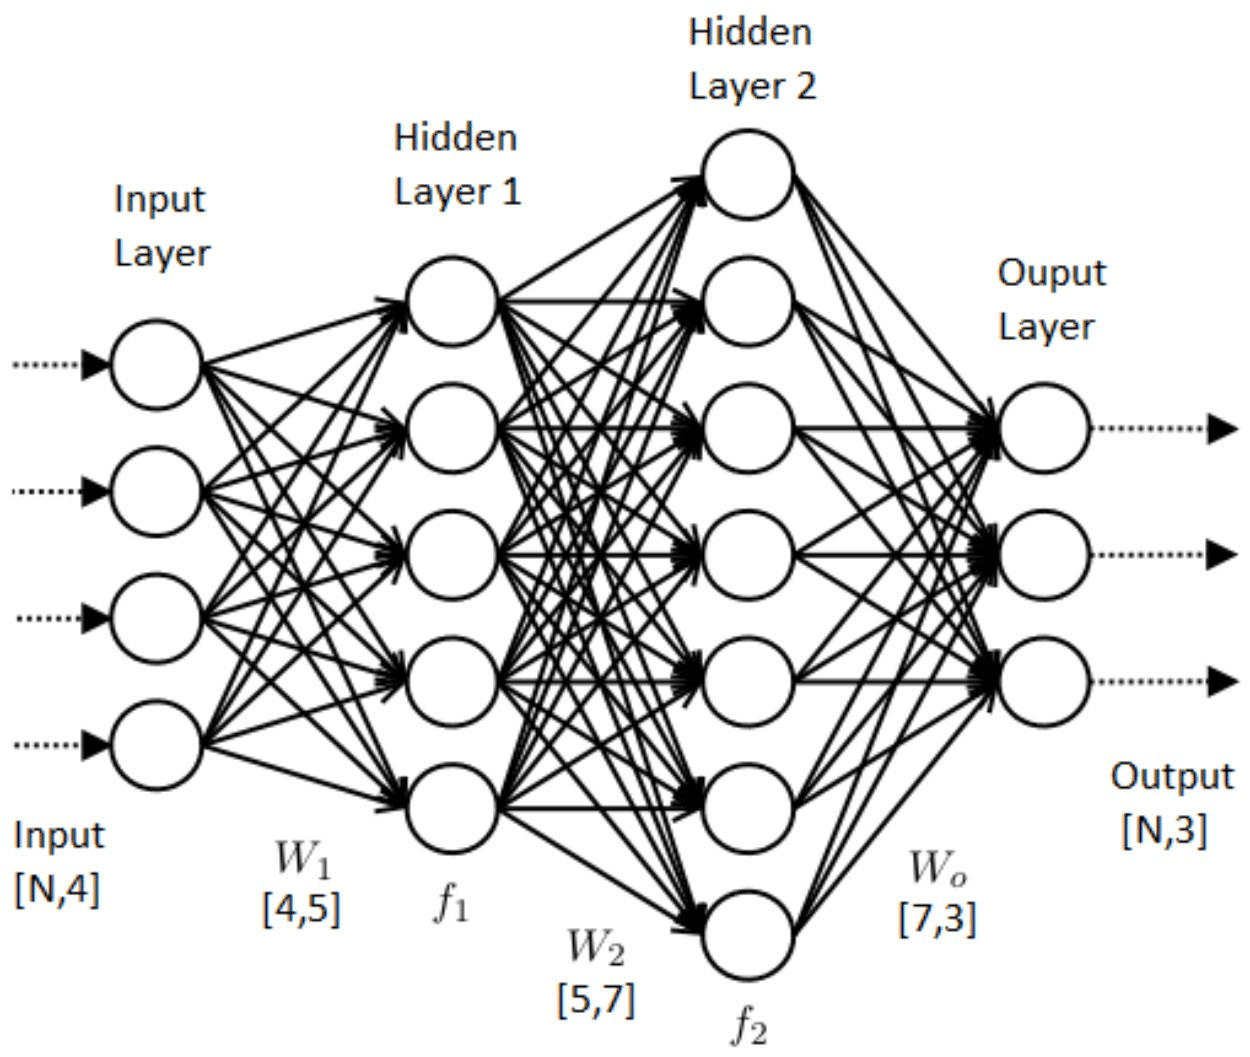
\includegraphics[height=0.85\textheight]{dense_1} \\
    \normalsize
    Image Source: Public Domain
    \pnote{
    Classic Dense FF \\
    has some arbitrary nonlinear activation function
    }
\end{frame}

\subsection{Activation Functions}
\begin{frame}[c]{Common Activation Functions}
    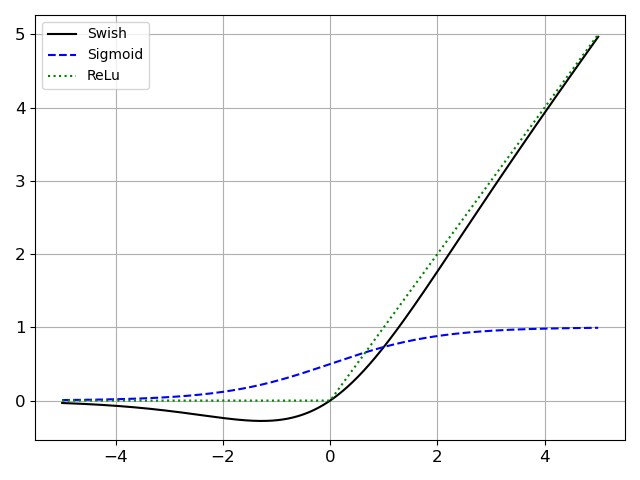
\includegraphics[height=0.75\textheight]{sigmoid_swish_relu} \\
    $swish(x) := x * sigmoid(x)$ \\
    Image Source: \cite{chen_deep_2021} \hspace{1cm}
    SwiGLU introduced by \cite{shazeer_glu_2020}
\end{frame}

\subsection{Dropout}
\begin{frame}[c]{Dropout}
    \begin{itemize}
        \item Problem: neural networks were rather 'unstable'
        \item solution: randomly 'deactivate' neurons during training
        \item this has the effect of the network not being overly reliant on individual neurons for certain features
        \item in effect, this makes networks substantially more robust and learn more generalized features, as they need to rely on more than a single neuron
        \item during testing, usually all neurons are active and weighted slightly lower
        \item Powerful method for regularization during training
        \item Dropout \cite{srivastava_dropout_2014}
    \end{itemize}
\end{frame}

\subsection{Residual Connections}
\begin{frame}[c]
    Skipping connections to propagate gradients
    Residual Connections \cite{he_deep_2016}
\end{frame}

\subsection{RegNet}

\begin{frame}[c]
    Self-Regulated Network \cite{xu_regnet_2021}
\end{frame}


\section{Embedding}
\subsection{Input}
\begin{frame}[c]
    \begin{itemize}[<+(1)->]
        \item Build Vocabulary
        \item Define Embedding Dimensions
        \item Learn Mapping
    \end{itemize}
\end{frame}

\subsection{Location}
\begin{frame}[c]
    Basically sinosoidal grid-cell patterns \\
    Simply getting added on top
\end{frame}


\section{Attention}

\subsection{Basic Attention}
\begin{frame}[c]
    Attention before Transformers \\
    Something about Q, K, V matrices and effects \\
    Yes we have empty context
\end{frame}

\subsection{Multi-Head Attention}
\begin{frame}[c]
    Multi-Head-Attention
\end{frame}

\subsection{Masked Attention}
\begin{frame}[c]
    Masking Attention
\end{frame}


\section{Transformer}

\subsection{Output}
\begin{frame}[c]
    FF and Softmax over embedding \\
    followed by topk selection
\end{frame}

\subsection{Putting it all Together}
\begin{frame}[c]
    Full Architecture Overview
\end{frame}

\subsection{Interpretation}
\begin{frame}[c]
    Solving PDE \cite{lu_understanding_2019}
\end{frame}

\subsection{Sparse Transformer}
\begin{frame}[c]
    Even the original GPT didn't use 'full' transformers, but Sparse Transformer \cite{child_generating_2019}
\end{frame}

\subsection{FastFormer}
\begin{frame}[c]
    Recently, people built a linear-cost attention mechanism: FastFormer \cite{wu_fastformer_2021}
\end{frame}

\subsection{Flash Attention}
\begin{frame}[c]
    Transformer Quality in Linear time \cite{hua_transformer_2022}
\end{frame}


\section{Compression}
\subsection{Quantization}
\begin{frame}[c]
    Reducing resolution of models after training significantly, e.g. from fp32 to fp8
\end{frame}

\subsection{Distillation}
\begin{frame}[c]
    Training a smaller model on outputting similar outputs distributions for given inputs
\end{frame}


\section{Successes}
\subsection{BERT}
\begin{frame}[c]
    generating language embeddings for NLP tasks
\end{frame}

\subsection{GPT2}
\begin{frame}[c]
    because architecture parameters and dimensions are known
\end{frame}

\subsection{CLIP}
\begin{frame}[c]
    Building semantic embeddings shared from pictures and text
\end{frame}

\subsection{Diffusion}
\begin{frame}[c]
    Generating images based on shared semantic embeddings
\end{frame}

\subsection{Physics Simulation}
\begin{frame}[c]
    Speed up simulation by 150x \cite{wiewel_latent_2019}
\end{frame}
